% \documentclass{article}
% \usepackage[utf8]{inputenc}
% \usepackage{fullpage}
% \usepackage{setspace}
% \usepackage[hang,flushmargin]{footmisc} %control footnote indent
% \usepackage{url} % for Appendicessite links
% \usepackage{amssymb,amsmath}%for matrix
% \usepackage{graphicx}%for figure
% \usepackage{appendix}%for appendix
% \usepackage{float}
% \floatstyle{plaintop}
% \restylefloat{table}
% \usepackage{multirow}
% \usepackage{longtable}
% \usepackage{morefloats}%in case there are too many float tables and figures
% \usepackage{caption}
% \usepackage{subcaption}
% \usepackage{listings}
% \captionsetup[subtable]{font=normal}
% \usepackage{color}
% \usepackage{hyperref}
% \usepackage[round]{natbib}
% \usepackage{rotating} % rotate table by some degree
% \usepackage{rotfloat}



% %\usepackage{Sweave}
% \setlength{\parindent}{0em}
% \setlength{\parskip}{0.5em}


% \graphicspath{{0.plots/}}



% \begin{document}

%%%%%%%%%%%%%%%%%%%%%%%%%%%%%%%%%%%%
\subsection{Simulation Studies} \label{sec:simulation}
%%%%%%%%%%%%%%%%%%%%%%%%%%%%%%%%%%%%
We conduct two simulation studies to validate the proposed QRJM. In the first simulation study, we assess the performance of the proposed Bayesian method in terms of bias and precision of the parameter estimates. In the second simulation study, we assess the predicted survival probability by comparing with the ``gold standard'' calculated based on the true (simulated) values of random effects and parameters.

%%%%%%%%%%%%%%%%%%%%%%%%%%%%%%%%%%%%
\subsubsection{Simulation Study I: Inferential Performance }\label{sec:sim1}
%%%%%%%%%%%%%%%%%%%%%%%%%%%%%%%%%%%%
In this simulation study, we consider different simulation scenarios where the random errors are generated from either a standard normal distribution or ALD distributions at different quantile $\tau$. The simulated data are then fitted using our proposed QRJM (assuming ALD for the random errors) as well as the LMJM (assuming normality for the random errors).


We let the covariate vectors in Model \eqref{eqn:joint} be ${\boldsymbol Z}_i(t)=(1, t)^{\top}, {\boldsymbol X}_i(t)=(1, x_{i1}, x_{i2}\cdot t)^{\top}, \mbox{ and } {\boldsymbol W}_{i}=(w_{i1}, w_{i2})^{\top}$ with covariates $x_{i1}, x_{i2}, w_{i1}$ and $w_{i2}$ being generated from independent standard normal distributions. We simulate the random effects, $\boldsymbol{u}_i$, from a bivariate normal distribution with mean vector {\bf 0}, and standard deviations both equal to 0.3 and correlation coefficient equals to 0.16.

To simulate the survival time, we choose constant baseline hazard. We obtain event time $T_i$ by inverting the survival function after generating $n$ random values from the standard uniform distribution. We generate the censoring time $C_i$ from $\textnormal{Beta}(4,1)$ to obtain a censoring proportion around 25\%. The longitudinal data are simulated from either a standard normal distribution or a ALD with the location parameter being $\boldsymbol{\beta}^{\top}{\boldsymbol X}_i(t) + {\boldsymbol u}_i^{\top}{\boldsymbol Z}_i(t)$ and dispersion parameter being $\sigma=1$. We keep a maximum of 6 observations for each subject, at follow-up time $t=(0, 0.25, 0.5, 0.75, 1, 3)$ respectively, after incorporating the time-to-event information.

We consider the following three scenarios in simulation study I:
\begin{enumerate}
\item Scenario 1: random errors follow the ALD with $\tau=0.25$ (right-skewed);
\item Scenario 2: random errors follow the ALD with $\tau=0.5$ (symmetric about 0 with heavy tails);
\item Scenario 3: random errors follow a standard normal distribution (symmetric about 0).
\end{enumerate}

In each scenario, we simulate 200 datasets with $N=600$ in each. Among the 600 subjects, we randomly select 500 subjects as the training dataset to build the model, and use the remaining 100 subjects as the validation dataset to make out-of-sample predictions.

We report bias, standard error (SE), mean squared error (MSE), and coverage probability (CP) for the QRJM and LMJM. Table~\ref{tab:sim1tab1} suggests that in Scenario 1, the true model (QRJM with $\tau=0.25$) provides parameter estimates with very small biases and CP being close to the nominal level. In comparison, the QRJM with $\tau=0.5$ provides reasonable estimates for most parameters, except the intercept $\beta_0$. The poor estimate of $\beta_0$ (large bias and CP far from 0.95) should not be surprising because of the incorrect specification of quantile $\tau$. The LMJM results in very biased estimates and the CP being away from the nominal value 0.95 (especially in regression parameters $\boldsymbol{\beta}$ in the longitudinal model). In Scenario 2 (see Appendices Table~\ref{tab:sim1tab2}) when data are symmetrical about 0 with heavier tails than the normal distribution, the LMJM still produces notably larger bias and lower CP as compared to the true model QRJM with $\tau=0.5$. In Scenario 3 (see Appendices Table~\ref{tab:sim1tab3}), median regression (the QRJM with $\tau=0.5$) performs comparably to the true model LMJM, suggesting that the QRJM can provide reasonable estimates when normality assumption holds. For completion, we also consider a scenario where the random errors are simulated from ALD with $\tau=0.75$ (left-skewed). The results (not presented) are very similar to Scenario 1, i.e., the true model QRJM with $\tau=0.75$ provides reasonable estimates while LMJM gives biased estimates and CP being far away from 0.95.
% latex table generated in R 3.2.2 by xtable 1.7-4 package
% Tue Oct 27 23:05:22 2015
\begin{table}[H]
% \begin{center}
\caption{Simulation results in Simulation study I Scenario 1 in which random errors are generated from ALD with $\tau=0.25$.}
\adjustbox{max width=\textwidth}{
\label{tab:sim1tab1}
\begin{tabular}{lrcccccccccccccc}
\hline
& \multicolumn{4}{c}{QRJM ($\tau=0.25$)} & & \multicolumn{4}{c}{QRJM ($\tau=0.5$)} & & \multicolumn{4}{c}{LMJM}\\
\hline
 & Bias & SE & MSE & CP && Bias & SE & MSE & CP && Bias & SE & MSE & CP \\
  \hline
  \multicolumn{10}{l}{Coefficients for longitudinal process} \\
  $\beta_0$ & $-$0.003 & 0.080 & 0.014 & 0.930 && 1.659 & 0.129 & 2.807 & 0.020 && 2.702 & 0.146 & 7.350 & 0.000 \\
  $\beta_1$ & 0.015 & 0.068 & 0.010 & 0.950 && 0.024 & 0.105 & 0.043 & 0.890 && 0.080 & 0.116 & 0.052 & 0.860  \\
  $\beta_2$ & 0.016 & 0.083 & 0.013 & 0.950 && 0.014 & 0.112 & 0.042 & 0.970 && 0.078 & 0.128 & 0.052 & 0.920  \\
  \multicolumn{10}{l}{Coefficients for survival process} \\
  $\gamma_1$ & 0.005 & 0.055 & 0.006 & 0.940 && 0.008 & 0.057 & 0.006 & 0.960 && 0.009 & 0.058 & 0.007 & 0.960  \\
  $\gamma_2$ & 0.006 & 0.055 & 0.006 & 0.930 && 0.010 & 0.056 & 0.007 & 0.910 && 0.010 & 0.058 & 0.007 & 0.940  \\
  $\alpha$ & $-$0.004 & 0.078 & 0.010 & 0.970 && $-$0.051 & 0.119 & 0.070 & 0.930 && $-$0.087 & 0.103 & 0.040 & 0.800  \\
   \hline
\end{tabular}
}
% \end{center}
\end{table}


%%%%%%%%%%%%%%%%%%%%%%%%%%%%%%%%%%%%
\subsubsection{Simulation Study II: Predictive Performance}\label{sec:sim2}
%%%%%%%%%%%%%%%%%%%%%%%%%%%%%%%%%%%%
In this simulation study, we make predictions for 100 subjects in the validation dataset (out-of-sample predictions) in the three scenarios in Section\ref{sec:sim1}. For each subject, we use the simulated data, random effects and the true parameter values to calculate the true survival probability given by $\frac{S_i[m|\mathcal{M}_{i}(m, {\boldsymbol u_i}, \boldsymbol{\theta});\boldsymbol{\theta}]}{S_i[t|\mathcal{M}_{i}(t, {\boldsymbol u_i}, \boldsymbol{\theta});\boldsymbol{\theta}]}$ and we use it as the ``gold standard''.

To assess the prediction validation (how well the models predict the survival probability), we use a Bland-Altman plot, a commonly used method to assess the agreement of the results from two measurement methods \citep{bland1986statistical}. To make the predictions ``dynamic'', we choose different combinations of censoring time (i.e., $t$) and the prediction time interval (i.e., $\Delta t$) to mimic expected real-world time points based on our HD data set. Appendices Figure~\ref{plot:sim2fig2} gives an intuitive comparison of the predicted results with the ``gold standard'' among different models. Plots from the true model (Appendices Figure~\ref{plot:sim2fig11}) are horizontally spindle-shaped, suggesting that it is easier to predict a probability near 0 or 1 than the middle probability area near 0.5. Further, with an increase in $\Delta t$, there is more variation in the middle probability area, indicating that survival probability predictions for time points further into the future are less accurate than predictions for closer time points, as expected. Bland-Altman plots from the other models (QRJM with $\tau=0.5$, Appendices Figure~\ref{plot:sim2fig12} and LMJM, Appendices Figure~\ref{plot:sim2fig13}) display systematically biased patterns in predictions.

Table~\ref{tab:sim2tab1} summarizes the comparison from the Bland-Altman plots for three chosen censoring time points ($t=0.25, 0.5, 0.75$). With longer follow-up time, we tend to have more longitudinal measurements per subject and tend to have more precise predictions.On the other hand, longer follow-up time leads to fewer subjects left in the study due to event occurrence and censoring (presented as a percentage in the first column of Table~\ref{tab:sim2tab1}), which results in higher variability in predictions. For example, in Table~\ref{tab:sim2tab1}, at $t=0.25$, there are 48.1\% subjects remain and at $t=0.5$ and 0.75, only 34.6\% and 22.8\%, respectively, of the subjects remain. As a result, we see comparable prediction results at $t=0.25$ and 0.5 but worse predictive performance when $t$ increases to 0.75. This is because the effect of additional longitudinal observations is ``canceled out'' by the variability from fewer subjects. Similarly, from the Bland-Altman plots, under the true model at the same censoring time $t$, an increase in $\Delta t$ leads to larger bias and MSE (Appendices Figure~\ref{plot:sim2fig11}). Because Table~\ref{tab:sim1tab1} suggests that the predictions from other models (QRJM with $\tau=0.5$ and LMJM) are systematically biased, their MSE and bias in Table~\ref{tab:sim2tab1} are much larger than the true model QRJM with $\tau=0.25$. Prediction results for Scenario 3 can be found in Appendices Table~\ref{tab:sim2tab2} and Appendices Figure~\ref{plot:sim2fig2}, in which QRJM with $\tau = 0.5$ performs comparably well as the true model when random errors are generated from standard normal distribution.

In summary, when data are simulated from ALD with specific skewness $\tau$, the best predictions of survival probability are obtained using the QRJM model with the exact quantile that generated the outcome data. Instead, LMJM results in systematically biased predictions when data are skewed. When random errors are standard normally distributed, predictions from QRJM with $\tau=0.5$ are comparable with those from the true model.

\begin{table}[H]
\centering
\caption{Simulation study: MSE and bias of the difference between predicted survival probability and the gold standard (Scenario 1).}
\adjustbox{max width=\textwidth}{
\label{tab:sim2tab1}
\begin{tabular}{clcccccccc}
\hline
 & & \multicolumn{2}{c}{QRJM ($\tau=0.25$)} & &\multicolumn{2}{c}{QRJM ($\tau=0.5$)} & &\multicolumn{2}{c}{LMJM} \\
\cline{3-4}\cline{6-7}\cline{9-10}
$t$ & $\Delta t$ & MSE & Bias & & MSE & Bias & & MSE & Bias \\
\hline
\multirow{2}{*}{{\bf 0.25}} & 0.25 & 0.006 & 0.009 && 0.137 & $-$0.330 & & 0.244 & $-$0.462 \\
&  1 & 0.010 & 0.007 && 0.111 & $-$0.267 & & 0.177 & $-$0.343 \\
\multirow{2}{*}{(subjects left: 48.1\%)} &  2 & 0.012 & 0.003 && 0.083 & $-$0.197 & & 0.126 &$-$0.249 \\
&  3 & 0.013 & 0.000 && 0.072 & $-$0.168 & & 0.107 & $-$0.210 \\
\hline
\multirow{2}{*}{{\bf 0.5}} & 0.25 & 0.007 & 0.009 && 0.130 & $-$0.317 & & 0.219 & $-$0.439 \\
&   1 & 0.015 & 0.000 && 0.144 & $-$0.321 & & 0.221 & $-$0.408 \\
\multirow{2}{*}{(subjects left: 34.6\%)}&   2 & 0.017 & $-$0.015 && 0.121 & $-$0.259 & & 0.174 & $-$0.319 \\
&   3 & 0.018 & $-$0.023 && 0.109 & $-$0.228 & & 0.153 & $-$0.278\\
\hline
\multirow{2}{*}{{\bf 0.75}} & 0.25 & 0.009 & 0.005 && 0.125 & $-$0.301 & & 0.189 & $-$0.401 \\
& 1 & 0.023 & $-$0.007 && 0.174 & $-$0.356 & & 0.253 & $-$0.447 \\
\multirow{2}{*}{(subjects left: 22.8\%)} & 2 & 0.025 & $-$0.033 && 0.159 & $-$0.310 & & 0.218 & $-$0.375 \\
&  3 & 0.027 & $-$0.046 && 0.148 & $-$0.282 & & 0.197 & $-$0.336\\
\hline
\end{tabular}
}
\end{table}






% \begin{figure}[H]
% \centering
% 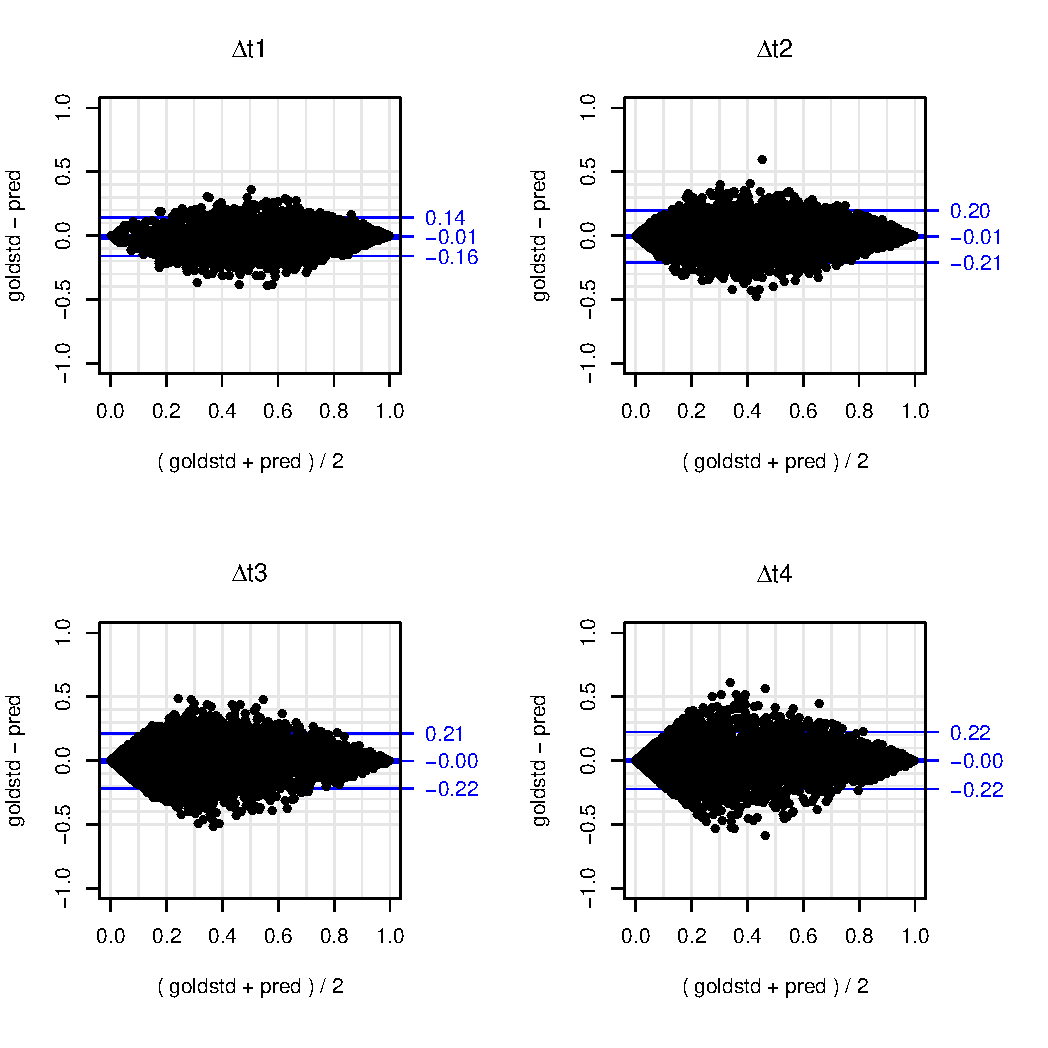
\includegraphics[width=0.45\textwidth]{baplot_qt25data_qt25fit_jags_t1.pdf}
% 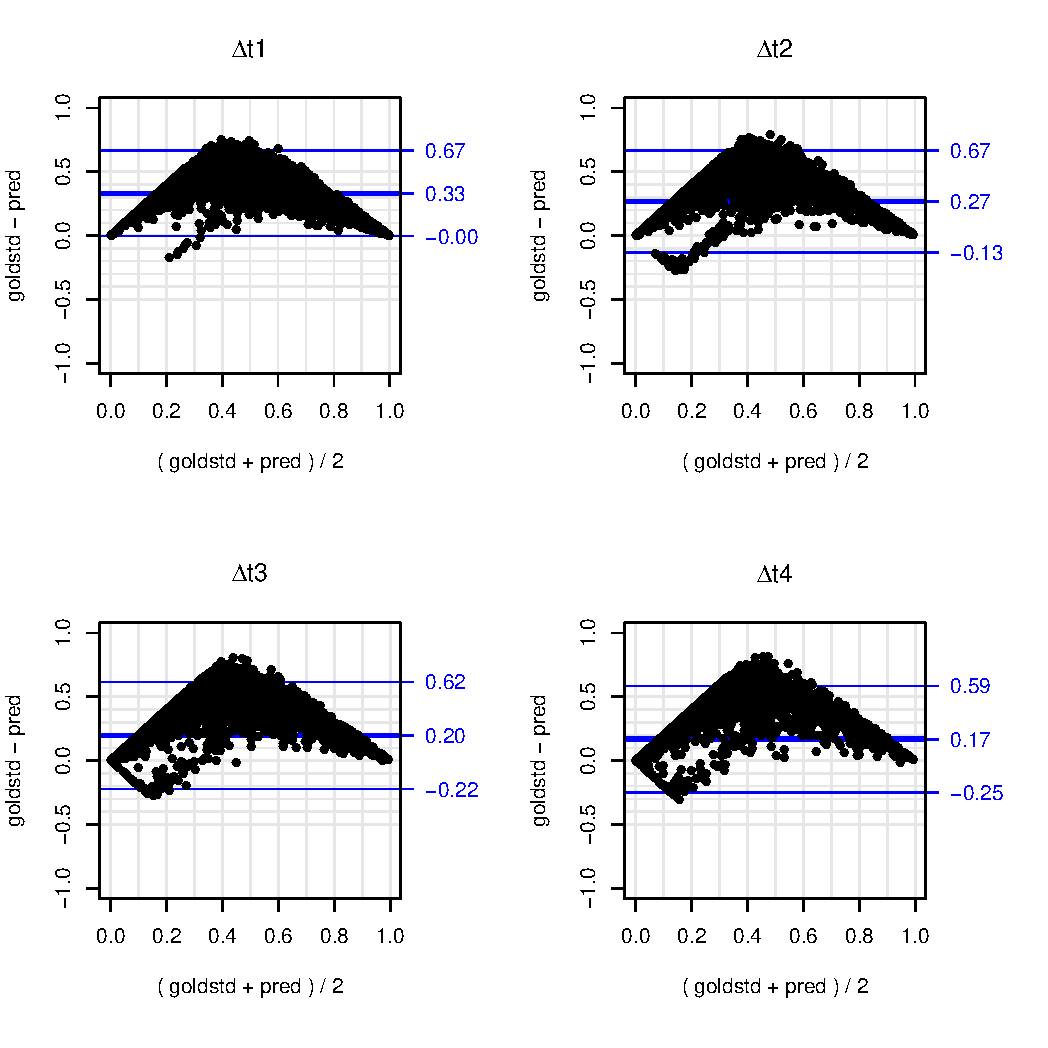
\includegraphics[width=0.45\textwidth]{baplot_qt25data_qt50fit_jags_t1.pdf}
% \hline
% 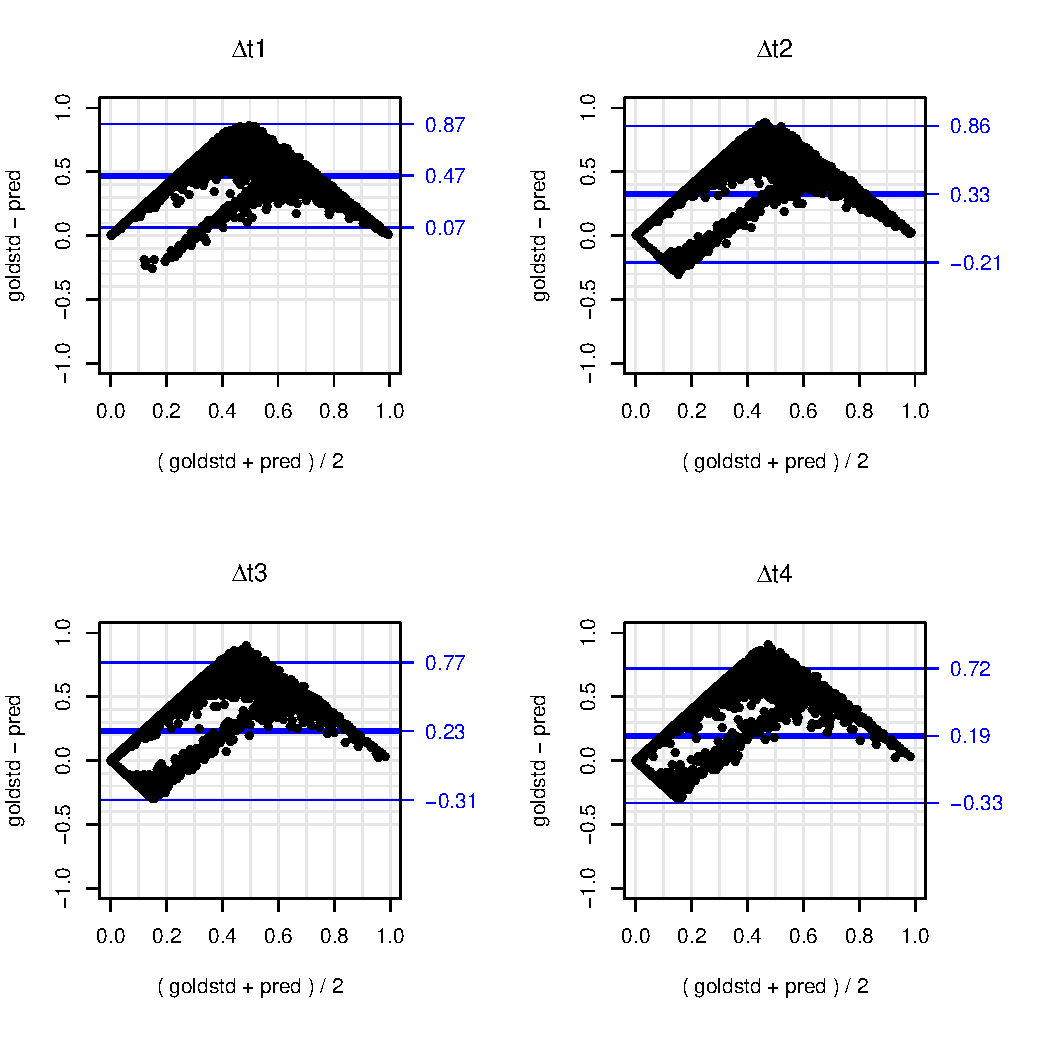
\includegraphics[width=0.45\textwidth]{baplot_qt25data_LMJMfit_arms_t1.pdf}
% \includegraphics[width=0.45\textwidth]{baplot_qt25data_JMbayesfit_t1.pdf}
% \label{plot:sim2fig1}
% \caption{BA plot of predictions with first two longitudinal observations ($t$=0.25) from true model (top left), QRJM with $\tau=0.5$(top right), LMJM (bottom left) and \LMJM(bottom right), Scenario One}
% \end{figure}










%
%
%All is done in \LaTeX \cite{knuth1986texbook}.
%
%
% \bibliographystyle{plainnat}%%%%%%%%%%%%%%%%%%%%
% \addcontentsline{toc}{section}{References}
% \bibliography{QRJM}

% \end{document}